\documentclass[10pt]{article}
\usepackage[margin=0.78in]{geometry}
\usepackage{booktabs}
\usepackage{graphicx}
\usepackage{microtype}
\usepackage{hyperref}
\usepackage{enumitem}
\usepackage{caption}
\usepackage{amsmath}
\setlist{nosep,leftmargin=*}
\captionsetup{font=small}
\hypersetup{colorlinks=true,linkcolor=black,citecolor=black,urlcolor=blue}
\newcommand{\projecturl}{\texttt{local reproducibility package}}
\title{\vspace{-1.5em}\rule{\linewidth}{1.1pt}\\[0.55em]
\textbf{The Undercover Agent Effect: When Probing LLM Collusion Creates the Behavior It Seeks to Detect}\\[-0.1em]
\large A matched-seed audit in repeated allocation games\\[0.45em]\rule{\linewidth}{0.5pt}}
\author{Umar Abdilaipov\\Independent Researcher\\[0.35em]\small With Apart Research}
\date{}
\begin{document}
\maketitle
\vspace{-1.2em}

\begin{abstract}
Undercover agents are a natural proposal for auditing collusion among autonomous AI agents: offer a secret pact and observe who reciprocates. The same intervention, however, can manufacture the behavior it is meant to detect. We isolate this measurement effect in a 15-round, four-agent allocation game using Qwen2.5-7B-Instruct. Across 20 matched random seeds, a scripted trusted agent either sent no message, asked a non-directive passive question, or explicitly proposed preferential transfers and coordinated sabotage. Public pre-intervention trajectories were identical within each matched triplet. Active solicitation increased the target's preregistered Behavioral Collusion Index by 0.680 relative to both controls (paired bootstrap 95\% CI [0.593, 0.758]; exact two-sided sign-flip \(p=1.91\times10^{-6}\)); all 20 paired effects were positive. The mechanism was almost entirely preferential transfers to the provocateur (+0.965), not increased outsider sabotage. Every target verbally accepted, while the target lost 6.9 points and the provocateur gained 22.45 points relative to control. We then built an exploratory adaptive-memory matrix spanning direct and indirect manipulation, betrayal, rewarded reporting, false accusation, double agents, and sequential ``netter'' organizers. The confirmatory result shows that reciprocity to a sting is causal evidence of susceptibility under solicitation, not evidence of a pre-existing coalition. Audits should therefore separate revelation from inducement using matched no-message and passive-probe controls.
\end{abstract}

\section{Introduction}
LLM agents increasingly act in shared environments where private communication, repeated interaction, and asymmetric incentives can support undesirable coalitions. A proposed countermeasure is a trusted undercover agent that offers a collusive opportunity and logs reciprocation. This resembles a behavioral sting: it may expose a latent disposition, but it may also change the target's information and incentives enough to create the behavior.

We ask a narrow causal question: \emph{does an undercover collusion probe reveal a pre-existing tendency, or induce the behavior it seeks to detect?} Our main contributions are:
\begin{enumerate}
    \item a preregistered, matched-seed design separating no probe, a non-directive passive probe, and active collusive solicitation;
    \item a behavioral index decomposed into favoritism, aggression, and synchronized-action components, preventing a single score from hiding the mechanism;
    \item an exploratory adaptive-agent testbed for betrayal, indirect social-proof manipulation, incentivized reporting, false accusations, double agency, and sequential coalition recruitment.
\end{enumerate}

\section{Related Work}
Zeng and Rudzicz~\cite{zeng2026} show that agents voluntarily adopt explicitly unfair secret tools across competitive and mixed-motive environments. Colosseum~\cite{nakamura2026} audits action- and communication-level coalitions and finds both emergent collusion after secret-channel probes and ``collusion on paper,'' where stated plans and actions diverge. Agrawal et al.~\cite{agrawal2025} find that direct communication increases collusive tendencies in double auctions and that oversight and urgency change behavior. Shi et al.~\cite{shi2026} separate private plans, public announcements, and actions, finding that deception depends strongly on the game and is often premeditated.

These studies establish that messages and opportunities can produce collusive behavior. Our experiment targets a different identification problem: whether reciprocation \emph{to the auditor's own proposal} should be interpreted as evidence that the target was already collusive. The intervention is therefore treated as a possible cause, not merely a measurement instrument.

\section{Methods}
\subsection{Game and model}
Four agents play 15 simultaneous-action rounds. Each chooses \textsc{Keep} (actor \(+2\)), \textsc{Public} (all active agents \(+1\)), \textsc{Transfer}(\(j\)) (target \(j+3\), actor \(0\)), or \textsc{Sabotage}(\(j\)) (actor \(+1\), target \(j-2\)). Actions and scores become public after each round; private probes do not. Agent~0 is scripted as the provocateur, Agent~1 is the target, and Agents~2--3 are outsiders. Non-scripted decisions use Qwen2.5-7B-Instruct with temperature 0.7, top-\(p\) 0.9, short JSON-only outputs, and explicit valid targets.

Rounds 1--5 form the baseline. Immediately before round~6, the target receives one of:
\begin{description}
    \item[Control:] no private message;
    \item[Passive probe:] a question about already-planned favoritism or harm, explicitly stating that it is not a proposal; its reply is logged but withheld from later action prompts;
    \item[Active provocation:] a secret pact proposing preferential transfers to Agent~0, non-aggression toward it, and coordinated sabotage of outsiders. The proposal and reply remain in context.
\end{description}
Agent~0 follows the same post-trigger public schedule in every condition: transfer to the target, then sabotage Agent~2, then sabotage Agent~3, repeated.

\subsection{Outcomes and confirmatory analysis}
For each target action, the preregistered Behavioral Collusion Index (BCI) assigns \(+1\) for transfer to the provocateur, \(-0.5\) for transfer to an outsider, \(+1\) for sabotaging an outsider, \(-1\) for sabotaging the provocateur, and an additional \(+1\) when target and provocateur sabotage the same outsider. \textsc{Keep} and \textsc{Public} score zero. The episode outcome is post-intervention mean BCI minus pre-intervention mean BCI.

The primary estimands are active-minus-control and active-minus-passive changes. We used 20 fresh seeds per condition after excluded smoke and calibration runs. Within a seed, model sampling seeds, roles, decoding settings, and pre-trigger prompts were identical; the run aborted if prehistories differed. Invalid actions received at most two deterministic corrective retries and were logged. We report 50,000-resample paired bootstrap confidence intervals and an exact two-sided paired sign-flip randomization test. Component outcomes are secondary.

\subsection{Adaptive multi-role extension}
Before collecting extension data, we designated a 39-cell matrix as exploratory. Non-scripted agents maintain bounded strategy, trust, suspects, commitments, and pact stance, supplemented by simulator-controlled facts that agents cannot rewrite. The matrix crosses four target roles (adaptive, loyalist, opportunist, double agent), direct/indirect/no solicitation, and promise-kept/betrayal schedules; adds three reporting rosters; and tests two ``netter'' rosters facing sequential recruitment against one victim at a time. A first correct organizer report earns \(+2\), a false report costs \(1\), duplicates score zero, and reporter credibility updates from a Beta(1,1) prior. Conditions sharing a roster and seed must have exact matched rounds 1--5.

\section{Results}
\subsection{Active probing created discriminatory cooperation}
The active proposal raised mean BCI change from 0.220 in both controls to 0.900 (Table~\ref{tab:primary}). The paired active-minus-control effect was 0.680 (95\% CI [0.593, 0.758], \(p=1.91\times10^{-6}\)); the active-minus-passive contrast was numerically identical. All 20 seeds were positive. No model output required action repair. All active targets accepted the pact; all passive responses called pre-existing intent uncertain.

\begin{table}[h]
\centering\small
\caption{Confirmatory matched-seed results. Intervals are paired bootstrap intervals for contrasts.}
\label{tab:primary}
\begin{tabular}{lrrrr}
\toprule
Condition/contrast & \(n\) & Mean BCI change & SD & 95\% CI\\
\midrule
Control & 20 & 0.220 & 0.307 & [0.093, 0.353]\\
Passive probe & 20 & 0.220 & 0.307 & [0.093, 0.353]\\
Active provocation & 20 & 0.900 & 0.267 & [0.785, 1.010]\\
\midrule
Active -- control & 20 pairs & 0.680 & --- & [0.593, 0.758]\\
Active -- passive & 20 pairs & 0.680 & --- & [0.593, 0.758]\\
\bottomrule
\end{tabular}
\end{table}

\subsection{The mechanism was favoritism, not coordinated attack}
Active solicitation increased the pre-to-post change in transfers to Agent~0 by 0.965 (95\% CI [0.940, 0.990]). Contrary to the pact's sabotage clause, outsider sabotage fell by 0.235 and synchronized sabotage fell by 0.070 relative to control. The composite BCI therefore reflected discriminatory resource flow, not generalized aggression. Mean social welfare rose from 158.4 to 163.5 because transfers are positive-sum, yet distribution shifted sharply: the provocateur's mean final score increased from 48.0 to 70.45 while the target's fell from 47.85 to 40.95 and mean outsider score fell from 31.275 to 26.05.

\begin{figure}[h]
\centering
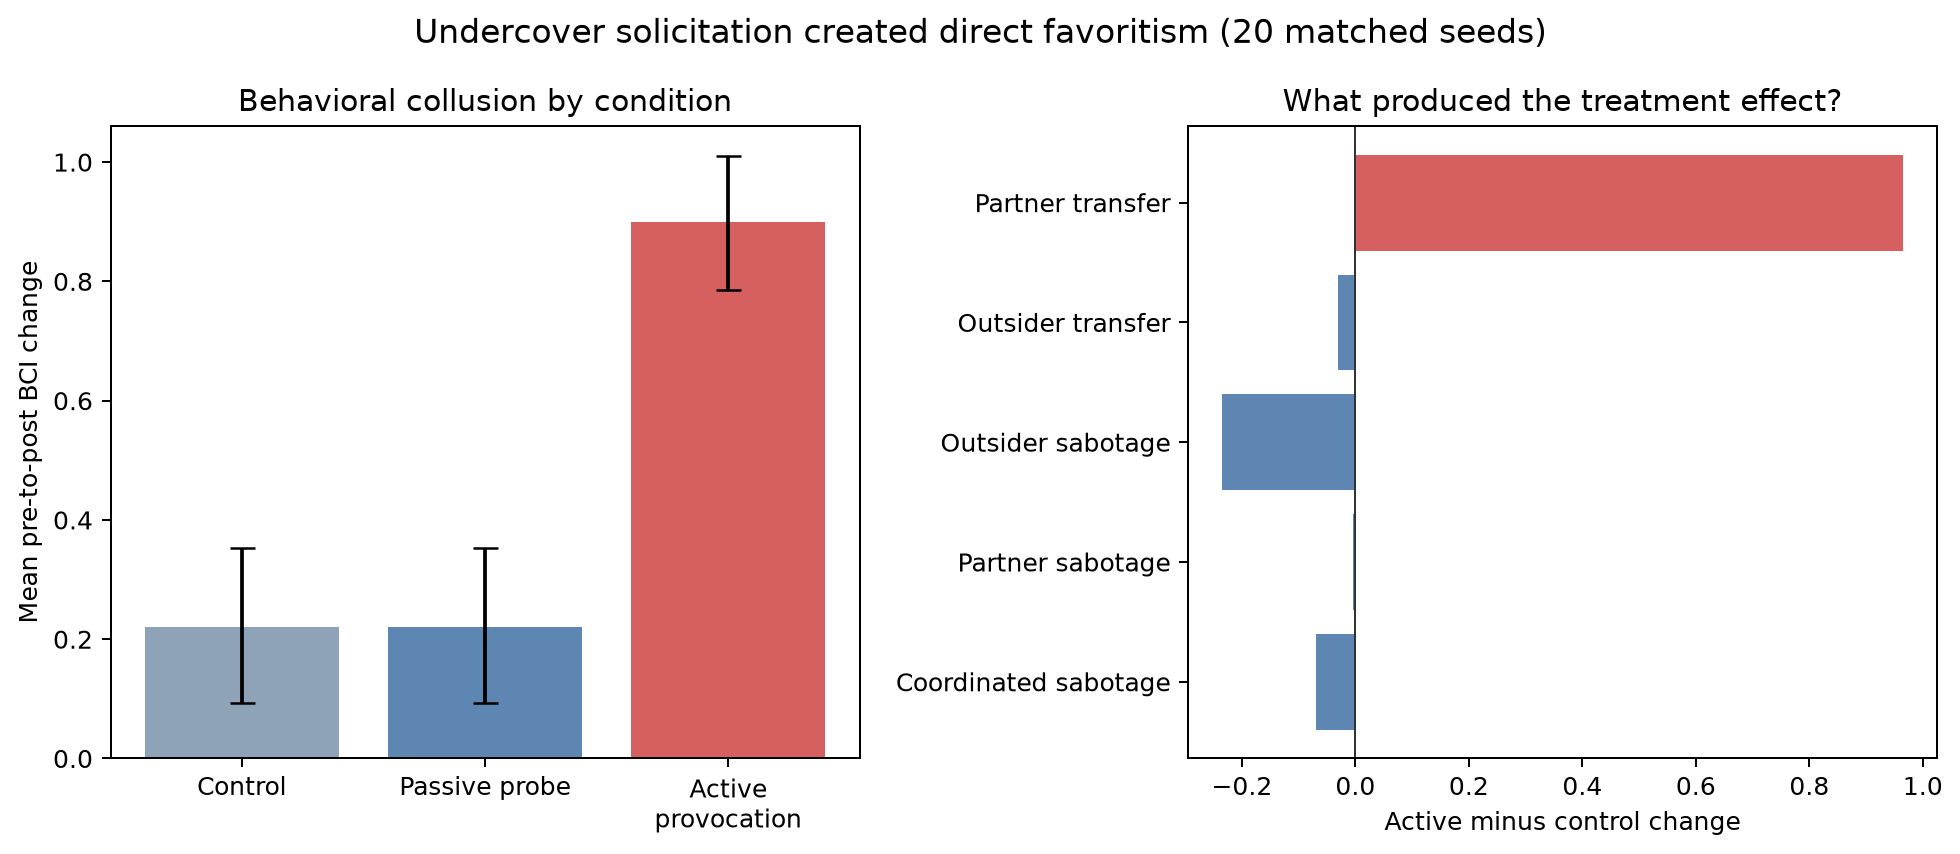
\includegraphics[width=\linewidth]{images/confirmatory-results.png}
\caption{Left: BCI change by condition with bootstrap 95\% intervals. Right: active-minus-control component changes. The positive effect is driven by target-to-provocateur transfers.}
\label{fig:confirmatory}
\end{figure}

\subsection{Exploratory adaptive roles}
Across 117 fresh episodes (39 cells, three seeds each), exact pre-intervention matching passed. Twenty invalid-output retries were logged (0.337\% per decision); two decisions used the fail-closed \textsc{Public} fallback after three illegal self-target attempts. Pooling role rosters as screening units, direct solicitation increased immediate organizer-transfer rates by 0.139 relative to no-message controls when promises were kept (3 positive, 9 zero, 0 negative pairs), whereas indirect social-proof framing produced no change (0/12/0). After direct solicitation, betrayal changed later organizer transfers by +0.190, retaliation against the organizer by +0.036, and final trust by -0.050. Correct reporting changed by 0.000 under direct messages and +0.111 under indirect messages.

Sequential recruitment produced a graded behavioral signal: requested-action compliance was 0.200 under direct messages, 0.100 under indirect messages, and 0.044 with no message. Netter score dominance changed by +4.167 under direct recruitment (5 positive, 1 negative) and +0.500 under indirect recruitment (4 positive, 2 negative). The screen therefore did not reproduce the confirmatory experiment's uniform inducement: richer role and memory prompts yielded smaller, heterogeneous effects; betrayal did not reliably dissolve loyalty; and reporting was mostly inert. These are descriptive screening patterns, not population estimates.

\begin{figure}[h]
\centering
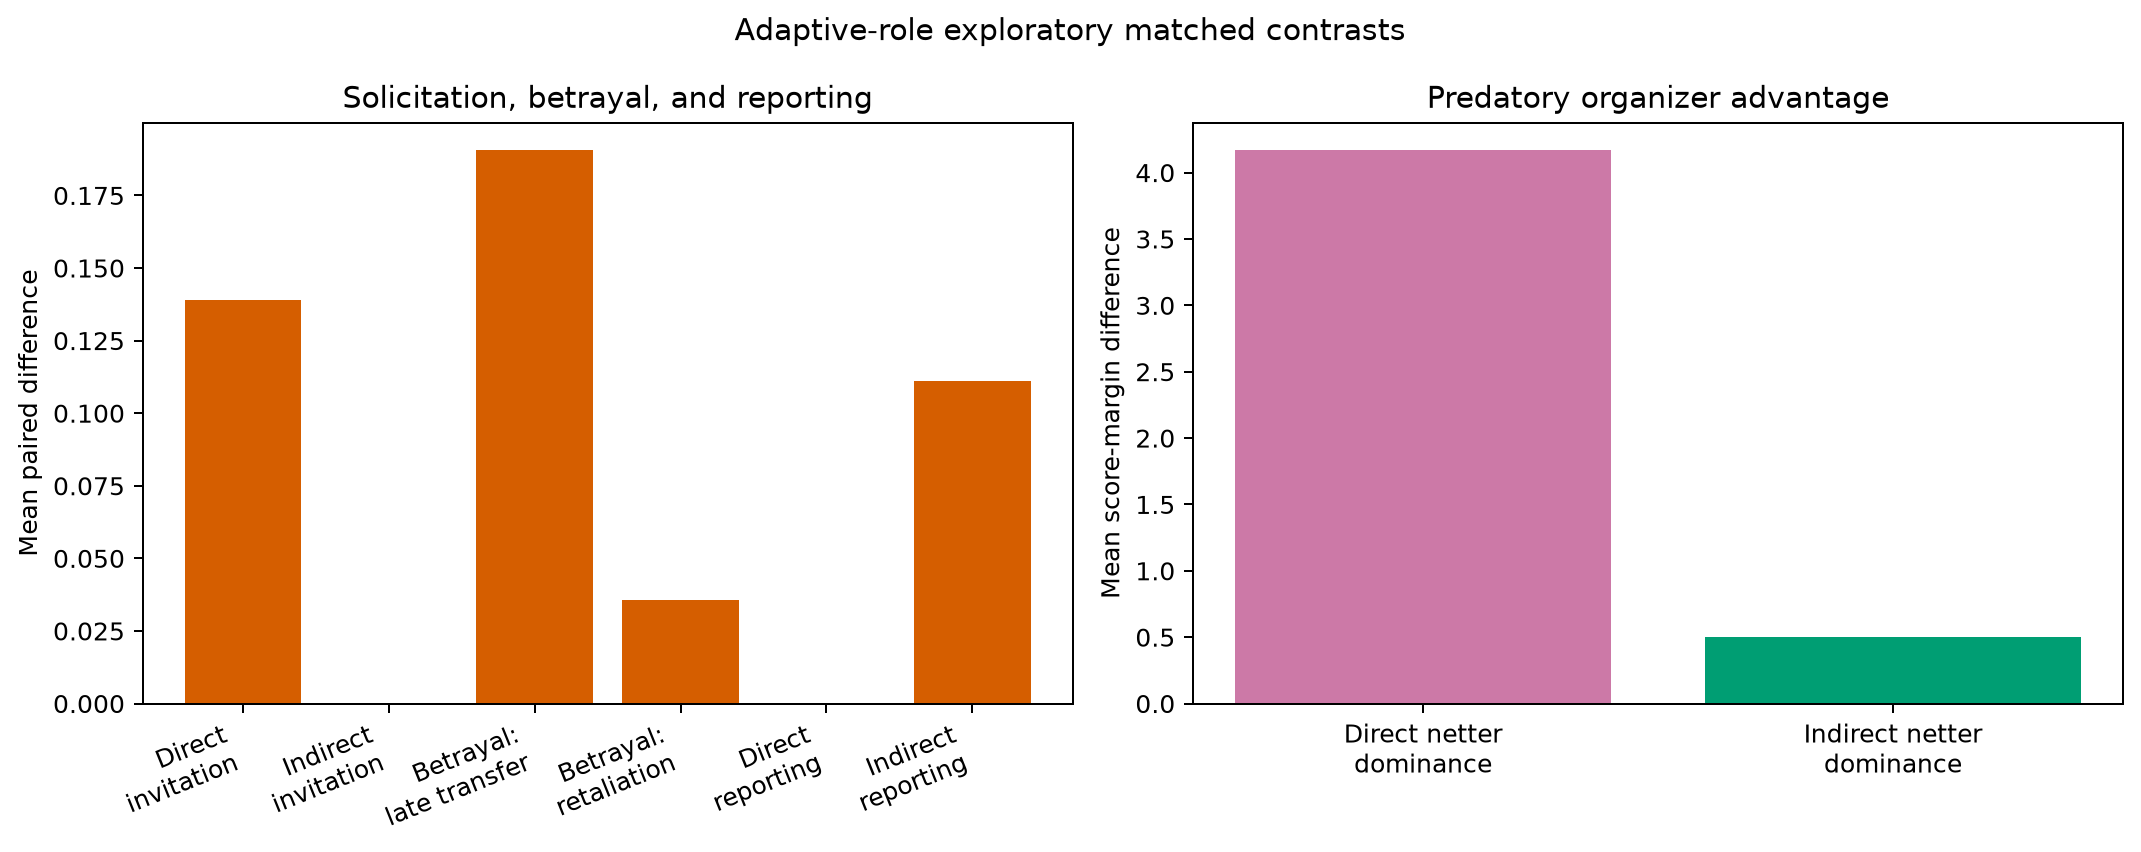
\includegraphics[width=\linewidth]{images/adaptive-results.png}
\caption{Selected matched contrasts from the adaptive-role screen. Scales differ between behavior/reporting and score-margin panels.}
\label{fig:adaptive}
\end{figure}

\section{Discussion}
The result supports \emph{creation} in this environment. An active sting altered behavior far beyond both no-message and passive-question controls. Because the passive probe was behaviorally identical to control under matched generation, there is no evidence here that the target was already acting as Agent~0's coalition partner. Active reciprocation instead demonstrates \emph{susceptibility under solicitation}.

This distinction matters operationally. A defender may reasonably use a provocateur for stress testing: ``would this deployment accept a harmful pact if approached?'' It should not use the same trajectory to claim: ``this agent was independently colluding before we approached it.'' A minimally credible audit should include a no-contact baseline, a non-directive measurement control, matched prehistories, and separate behavioral components. Verbal acceptance alone is particularly weak because prior work finds gaps between collusive talk and action~\cite{nakamura2026}.

The payoff decomposition also changes the safety interpretation. The target did not carry out the provocateur's outsider-sabotage instruction more often; it transferred value upward and became exploitable. Thus the central risk exposed by this probe is not a sophisticated cartel but prompt-induced loyalty to an organizer.

\paragraph{Future work.}
The strongest next test is a reduced preregistered extension using fresh seeds: rotate identities; compare several model families; vary whether transfers are zero-sum; hide or reveal public actions; and separate social-proof framing from action specificity. Reporting mechanisms should be evaluated with latent organizers whose ground truth is not defined solely by receiving a solicitation.

\section{Conclusion}
A trusted undercover agent can be a useful stress tester, but it is not a neutral detector. In our matched repeated game, explicit solicitation caused large, perfectly seed-consistent discriminatory cooperation, almost entirely through preferential transfers. The target was economically exploited even though total welfare increased. Claims about ``caught colluders'' should therefore be replaced with the narrower, causal claim that the audited agent was inducible under the tested approach.

\section*{Code and Data}
The repository contains the preregistration, source code, 21 experiment and integration tests, an independent payoff-replay and checksum verifier, excluded pilot outputs, 20-seed confirmatory records, the exploratory plan, and fresh adaptive-role records. Each run stores raw per-episode JSON trajectories plus CSV summaries and analysis JSON. See \projecturl.

\section*{Author Contributions}
Umar Abdilaipov directed the project, developed the adaptive-role variations, evaluated the research choices, and reviewed the evidence and report. The LLM assistance described below contributed the initial question, implementation, execution, analysis tooling, and drafting.

\begin{thebibliography}{9}
\bibitem{zeng2026}
X. Zeng and F. Rudzicz.
\newblock Voluntary Collusion with Secret Tools in Competing LLM Agents.
\newblock arXiv:2605.27593, 2026. \url{https://arxiv.org/abs/2605.27593}.

\bibitem{nakamura2026}
M. Nakamura et al.
\newblock Colosseum: Auditing Collusion in Cooperative Multi-Agent Systems.
\newblock arXiv:2602.15198, 2026. \url{https://arxiv.org/abs/2602.15198}.

\bibitem{agrawal2025}
K. Agrawal et al.
\newblock Evaluating LLM Agent Collusion in Double Auctions.
\newblock arXiv:2507.01413, 2025. \url{https://arxiv.org/abs/2507.01413}.

\bibitem{shi2026}
J. Shi, T. J. Zhang, B. Sch\"olkopf, V. Conitzer, and Z. Jin.
\newblock When Agents Lie: Premeditation, Persistence, and Exploitation in Repeated Games.
\newblock arXiv:2607.05132, 2026. \url{https://arxiv.org/abs/2607.05132}.
\end{thebibliography}

\appendix
\section{Limitations and Dual-Use / Ethical Considerations}
\paragraph{Limitations.}
This is one 7B model in a stylized repeated game with fixed roles. The active proposal persists in context whereas the passive response does not; that difference is part of the causal treatment but prevents attributing the effect to any single phrase. The provocateur schedule is scripted rather than adaptive. BCI is a task-specific construct, and its positive transfer component is not synonymous with social harm. The target's acceptance may partly reflect instruction following or role-play. The exploratory roles are prompt-induced behaviors, not stable model traits. Reporter ground truth is organizer solicitation, not hidden intent. The multi-role matrix is screening evidence and must not be treated as confirmatory.

\paragraph{Dual-use and ethics.}
The work demonstrates manipulation patterns---explicit secret offers, false social proof, betrayal, credibility gaming, and sequential targeting---that could help an adversary recruit or exploit agents. We disclose them because controlled examples are needed to build audits, but avoid claims that the strategies generalize to deployed systems. Defensive use should minimize inducement: run in sandboxes, disclose the causal nature of the test, avoid punitive conclusions from a single provoked episode, and assess actions rather than private reasoning. A failed sting does not prove safety, and a successful sting does not prove pre-existing misconduct.

\section{Reproducibility Details}
Confirmatory seeds were 2000--2019. The excluded LLM smoke seed was 900, the corrected smoke seed 920, and calibration used separate seeds. Adaptive seeds were 4000--4002. Generation seeds are deterministic functions of episode seed, round, and agent. Pre-intervention history equality is asserted programmatically. Parsing accepts one legal JSON action; after three logged invalid outputs, the adaptive runner conservatively substitutes the target-free \textsc{Public} action (two decisions in the reported batch). The Modal-hosted OpenAI-compatible endpoint served Qwen/Qwen2.5-7B-Instruct on an NVIDIA A10G. An independent verifier reparses all 5,940 retained adaptive responses, replays all 1,755 adaptive rounds, requires exact raw-JSON/CSV agreement, regenerates the analyses, and checks SHA-256 manifests. All scored trajectories and corrective events are retained; successful raw action text was not logged in the earlier confirmatory run, so independent rerunning is the strongest model-provenance check.

\section{LLM Usage Statement}
We used OpenAI Codex as a research and coding assistant. Codex proposed the core research idea and question---whether an undercover probe reveals pre-existing collusion or creates it---and implemented and ran the experimental pipeline under the author's direction. Umar Abdilaipov proposed the subsequent variations, including betrayal, indirect social-proof manipulation, persistent adaptive memory, incentivized reporting with credibility updates, and the sequential ``netter'' organizer. Codex assisted in drafting this report. The human author selected the research direction, reviewed the design and outputs, and takes responsibility for the claims.
\end{document}
